\documentclass[11pt,letterpaper,boxed]{../hmcpsetrhino}
\usepackage[margin=1in]{geometry}
\usepackage{graphicx}
\usepackage{enumerate}
\usepackage{amsthm}
\usepackage{amsmath}

\newcommand{\ds}{\displaystyle}
\newcommand{\half}{\frac{1}{2}}
\newcommand*\Eval[3]{\left.#1\right\rvert_{#2}^{#3}}
\newcommand{\eval}{\biggr\rvert}
\newcommand\Partial[2]{\frac{\partial #1}{\partial #2}}
\newcommand\mat[1]{\underline{\vec {#1}}}
\newcommand\tp[1]{\widetilde {#1}}
\def\EE{{\cal E}}
\def\Lagr{\mathcal{L}}
\def\Ham{\mathcal{H}}

\name{}
\class{Physics 111 Section 1}
\assignment{Problem Set 15}
\duedate{November 7, 2016}

\begin{document}

\problemlist{Oscillations: Damped Systems (Reading: Chapter 5.1 - 5.4)}
\textbf{Help:}

\begin{problem}[5.2]
The potential energy of two atoms in a molecule can sometimes be approximated by the Morse function,
\[	U(r) = A\left[\left(e^{(R-r)/S} - 1\right)^2 - 1\right]\]
where $r$ is the distance between the two atoms and $A$, $R$, and $S$ are positive constants with $S \ll R$. Sketch this function for $0 < r < \infty$. Find the equilibrium separation $r_0$, at which $U(r)$ is minimum. Now write $r = r_0 + x$ so that $x$ is the displacement from equilibrium, and show that, for small displacements, $U$ has the approximate form $U$ = const + $\half kx^2$. That is, Hooke's law applies. What is the force constant $k$?
\end{problem}
\begin{solution}


\vfill
\end{solution}

\newpage 


\begin{problem}[5.19]
Consider the mass attached to four identical springs, as shown in Figure 5.7(b). Each spring has force constant $k$ and unstretched length $l_0$, and the length of each spring when the mass is at its equilibrium at the origin is $a$ (not necessarily the same as $l_0$). When the mass is displaced a small distance to the point $(x, y)$, show that its potential energy has the form $\half k' r^2$ appropriate to an isotropic harmonic oscillator. What is the constant $k'$ in terms of $k$? Give an expression for the corresponding force.
\[	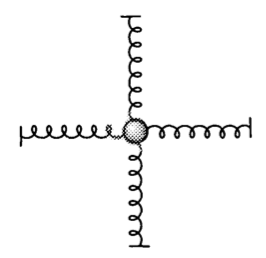
\includegraphics{fig1}\]

\end{problem}
\begin{solution}


\vfill
\end{solution}

\newpage 

\begin{problem}[5.25]
Consider a damped oscillator with $\beta < \omega_0$. There is a little difficulty defining the "period" $\tau_1$ since the motion (5.38) is not periodic. However, a definition that makes sense is that $\tau_1$ is the time between successive maxima of $x(t)$. 
\begin{enumerate}[(a)]
\item Make a sketch of $x(t)$ against $t$ and indicate this definition of $\tau$ on your graph. Show that $\tau_1 = 2 \pi / \omega_1$.

\item Show that an equivalent definition is that $\tau_1$ is twice the time between successive zeros of $x(t)$. Show this one on your sketch. 

\item If $\beta = \omega_0/2$, by what factor does the amplitude shrink in one period?

\end{enumerate}
\end{problem}
\begin{solution}


\vfill
\end{solution}

\newpage 


\begin{problem}[5.27]
As the damping on an oscillator is increased there comes a point when the name "oscillator" seems barely appropriate. 
\begin{enumerate}[(a)]
\item To illustrate this, prove that a critically damped oscillator can never pass through the origin $x=0$ more than once.

\item Prove the same for an overdamped oscillator.

\end{enumerate}
\end{problem}
\begin{solution}


\vfill
\end{solution}

\end{document}
